% chapter2.tex
%motivation of the analysis of long term measurement~~ Dark Matter->WIMP->EDEILWEISS->Background

Nowadays, the search for dark matter becomes one of the central topics in astroparticle physics.  Numerous experiments aim to search for dark matter. In this chapter, observational evidences of dark matter are given, followed by a description of particle candidates of dark matter with focus on WIMP. EDELWEISS is one of the experiments to directly search for dark matter. The general setup and working principle is described.

%enregieanteil durch CMB ,lambda-cdm,...
%outline for this chapter
%%%%%%%%%%%%%%%%%%%%%%%%%%%%%%%%%%%%%%%%%%%%%%%%%%%%%%%%%%%%%%%%%%%%%%%%%%%%%%%%
%%%%%%%%%%%%%%%%%%%%%%%%%%%%%%%%%%%%%%%%%%%%%%%%%%%%%%%%%%%%%%%%%%%%%%%%%%%%%%%%
\section{Evidences of dark matter}
In 1933, while studying on the velocity dispersion of galaxies inside the Coma galaxy cluster, F.Zwicky inferred the existence of some kind of unseen mass, which he called \textit{dunkle Materie} (dark matter). Since then, his idea was supported by numerous observations on different scales -- e.g. CMB, the Bullet Cluster.
The Bullet Cluster (1E 0657-56) consists of two clusters, which collided around $\SI{100}{Myrs}$ ago. Using gravitational lensing and X-Ray analysis, it is found that the two galaxy concentrations have moved ahead of their plasma clouds, which indicates the existence of weak-interacting dark matter.
In the following a more detailed description of evidence of dark matter in galaxy is given.
\subsection*{Galaxy rotation curve}
Take a simplified model with only the gravitation, the rotation velocity of an object at large distances from the galactic centre can be approximated:
\begin{equation}
  v(r)=\sqrt{\frac{GM}{r}}
\end{equation}
M denotes the galactic mass, and r the distance to the galactic centre. Therefore, the velocity is expected to be e$v \approx r^{-1/2}$ at large distances according to the Kepler's law. However, observation of flat rotation curves shows discrepency from the expectation. In 1980, an extensive study of 21 galaxies suggests that most stars in spiral galaxies have roughly the same oribit velocity, which implies the existence of some kinde of unseen matter \cite{Rub80}.
\begin{figure}[ht]
  \centering
  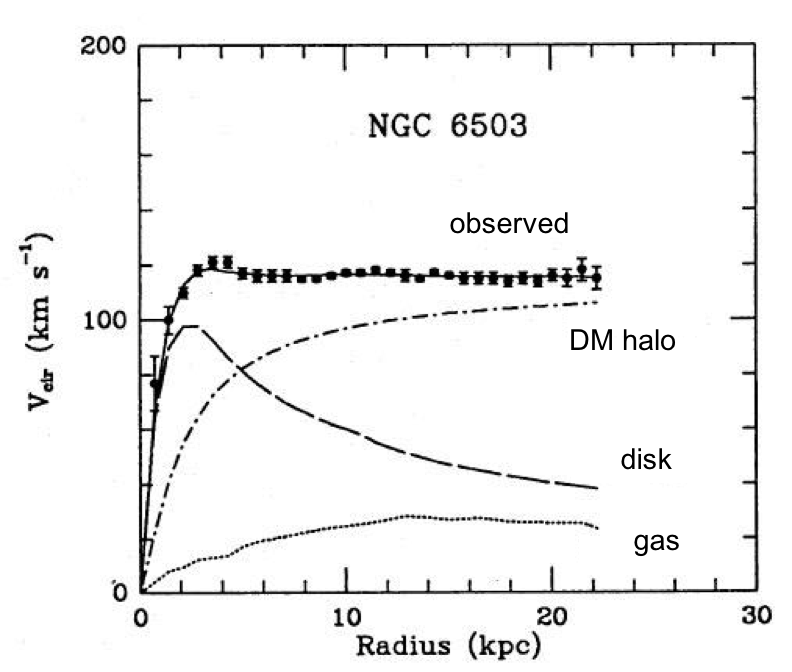
\includegraphics[width=0.75\textwidth{}]{./fig/rotation_curve.png}
  \caption{ An example of galaxy rotation curve (NGC 6503). The observed rotation curve is plotted with the individual components.
  . Extracted from \cite{Rub80}.}.
  \label{fig:rotation-curve}
\end{figure}
Fig \ref{fig:rotation-curve} shows an example of the observed rotation curve of one spiral galaxy. The contribution of baryonic matter (disk and gas) decreases with distance, whereas the DM-halo one rises. Together they lead to the observed flat curve at large radius.

It should also be mentioned that there are alternative theories to explain the problem of galaxy rotation curves, such as Modified Newtonian Dynamics (MOND). Although MOND successfully solves the problem in galactic scale, it cannot cope with the observations at larger scales.
%%%%%%%%%%%%%%%%%%%%%%%%%%%%%%%%%%%%%%%%%%%%%%%%%%%%%%%%%%%%%%%%%%%%%%%%%%%%%%%%
%%%%%%%%%%%%%%%%%%%%%%%%%%%%%%%%%%%%%%%%%%%%%%%%%%%%%%%%%%%%%%%%%%%%%%%%%%%%%%%%
%%%%%%%%%%%%%%%%%%%%%%%%%%%%%%%%%%%%%%%%%%%%%%%%%%%%%%%%%%%%%%%%%%%%%%%%%%%%%%%%

\section{WIMP as dark matter candidate}
The $\mathrm{\Lambda}$ cold dark matter($\mathrm{\Lambda}$CDM) model is a parametrization of the Big Bang model and successfully explains the evolution of the universe. It is therefore often referred to as the standard model of cosmology. As the name suggests, $\mathrm{\Lambda}$CDM model contains a cosmological constant (denoted with $\mathrm{\Lambda}$) and cold dark matter, which means that dark matter mostly consist of non-relativistic paricles. Also, dark matter is electrically uncharged and mostly collisionless. The DM particles only interact with itself and other particles through gravitation and weak force. They has to be stable, otherwise they would not exist with such abundance nowadays.

In standard model, no particle satisfies all the properties above. The standard model is thus to be extended. There are many hypothetical particles as potential dark matter candidates,e.g. Axions, sterile neutrinos, WIMPs. Axion is a hypothetical elementry particle to solve the strong CP problem \cite{Pec77}. Sterile neutrinos are right-handed neutrinos that only interact via gravitation. They would be candidate of warm dark matter if their mass is in keV range. The dark matter candidate of interest in this work is called WIMP (weakly inteacting massive particle), a generic class of hypothetical particles.

WIMP is expected to have mass of ~$\SI{100}{GeV}$ and inteact weakly and gravitationally.  For sufficiently high temperatures, like in the early universe, the WIMPs are constanly produced and annihilated. As the temperature drops, the WIMPs almostly cease to interact and the particle density remains roughly the same. A promising candidate of WIMP is the so-called lightest supersymmetric particle (LSP) of the supersymmetric model (SUSY). SUSY is a extension of the standard model that each SM-particle has a SUSY-partner which differs only by a half-integer spin. In many models the LSP turns out to be neutralino, which is the mixture of four SUSY-particles.

Due to the low interaction cross section, WIMPs are extremely hard to detect. They can be detected through different methods. They can be produced by collision of SM-particles. WIMPs can also be detected indirectly by measuring the SM-particles produced in self-annihilation of dark matter. Lastly, they can be directly detected by observation of WIMP-nucleus scattering like in EDELWEISS experiment.

%%%%%%%%%%%%%%%%%%%%%%%%%%%%%%%%%%%%%%%%%%%%%%%%%%%%%%%%%%%%%%%%%%%%%%%%%%%%%%%%
%%%%%%%%%%%%%%%%%%%%%%%%%%%%%%%%%%%%%%%%%%%%%%%%%%%%%%%%%%%%%%%%%%%%%%%%%%%%%%%%
%%%%%%%%%%%%%%%%%%%%%%%%%%%%%%%%%%%%%%%%%%%%%%%%%%%%%%%%%%%%%%%%%%%%%%%%%%%%%%%%

\section{EDELWEISS-III Experiment}
  \label{edw}
  The EDELWEISS experiment is dedicated to detect the scattering of WIMPs on ordinary matter at cryogenic temperature. In order to achieve the expected sensitivity down to \SI{e-9}{pb}, the main challenge is to exclude all the bacgrounds induced by radioactivity or cosmic rays. The general setup of the experiment and the possible backgrounds are summarized in section \ref{sec:edw-exp}. The remaining backgrounds can be discriminated by measurements of two channels of the signal. This working principle of Germanium Bolometers is briefly described in section \ref{edw-ge}.
  The problematic muon-induced neutrons, which cannot be distinguished from the WIMP-signal, is described in detail in chapter \ref{chap:muon}.
\subsection{Experimental setup and backgrounds at EDELWEISS}
  \label{sec:edw-exp}
  The EDELWEISS experiment is located in the underground laboratory of Mondane (\textit{Laboratoire Souterrain de Modane}, LSM). Under 1780 meters of rock, the cosmic muon flux is reduced by more than a factor \num{e6} to a reamaining rate of 5\,$\mathrm{\mu}$/$\mathrm{m}^{2}$/d \cite{Sch13a}.
  The remaining throughgoing muons are tagged with an active \mvs, which is the outermost layer of the setup. (see fig.\ref{fig:exp-setup}). A detailed description and working principle are given in chapter \ref{chap:muon}.

  \begin{figure}[ht]
    \centering
    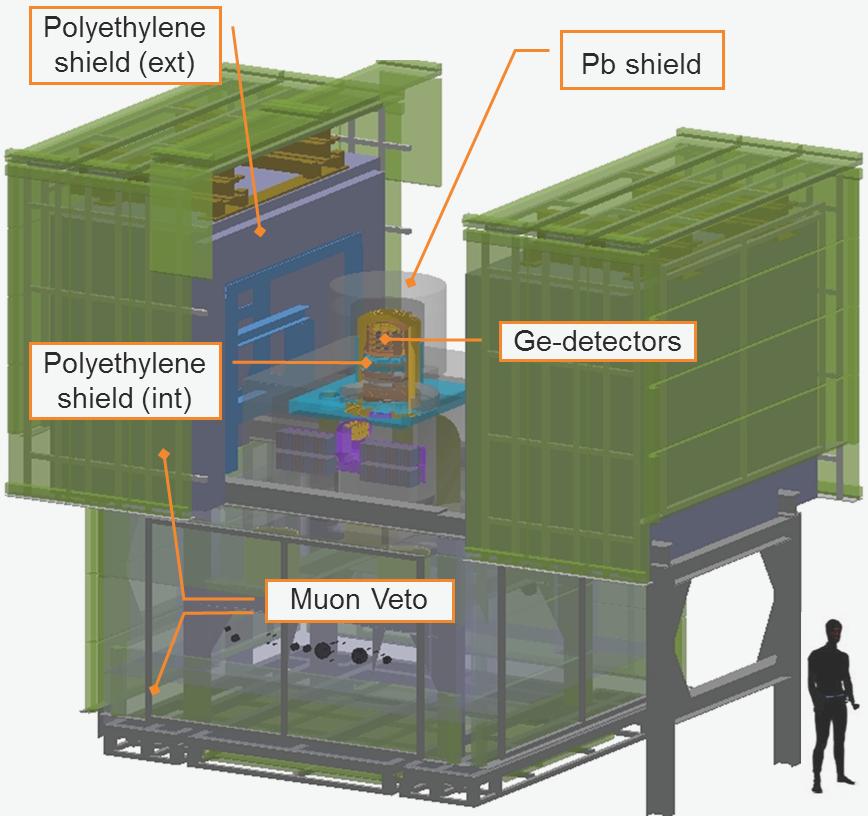
\includegraphics[width=0.75\textwidth{}]{./fig/exp_setup.png}
    \caption{\textbf{Schematic view of EDELWEISS experimental setup}.
    In the center are the Ge-bolometers hosted in a cryostat. The cryostat is surrounded by a lead shield, a PE shield and an active muon veto system to minimize the backgrounds.} Extracted from \cite{Kef16}.
    \label{fig:exp-setup}
  \end{figure}


  The next layer is a polyethylene (PE) shield of about \SI{50}{cm} thickness to attenuate the neutron flux from the radioactivity of rock and experiment materials. The fast neutron flux with energy above \SI{1}{MeV}, which produces similar recoils as from WIMPs, is reduced by 5 to 6 orders of magnitude. %\ref{backgrounds...}
  Next to the PE shield is a lead shield of 20 cm thickness to reduce the ambient $\upgamma$ background. The nature lead contains radioactive isotopes--e.g. \ce{^{210}Pb}, \ce{^{238}U} and \ce{^{232}Th}, which also contribute to the background. To reduce its natural raioactivity, the innermost \SI{2}{cm} of the shield is made of Roman lead discovered in a sunken ship. The \ce{^{210}Pb} has a half-life of $T_{1/2}=\SI{22}{years}$, so that it's abundance is decreased by two orders of magnitude \cite{Sch13a}.
  Another source of background is the \ce{^{222}Rn} as a decay product of \ce{^{238}U}.

  The upper part with the cryostat is installed in a clean room with renewing air to minimize the radon level. The space between the lead shield and the cryostat is flushed with filtered air.
  The upper part of the shieldings are mounted on rails and can be opened in halves to access the cryostat and electronics. Additional layers of PE and lead shields are installed inside the cryostat to reduce the background induced by electronics and cables.

  The cryostat is a \ce{^{3}He}/\ce{^{4}He} dilution refrigerator made of low-radioactivity materials. The detectors are enclosed in five thermal screens and the temperaturs decreases from room temperatur over \SI{100}{K}, \SI{40}{K}, \SI{4}{K}, \SI{1}{k} to \SI{10}{mK}. In standard operations, the temperature of the detectors is tuned to $T=(18.000 \pm 0.002)\,\si{mK}$.

\subsection{Working principle of Ge Bolometer}
  \label{edw-ge}
  The bolometers used in EDELWEISS experiment are made of high-purity monocrystalline germanium. They are equipped with aluminium ring electrodes and glued with 2 Neutron Transmutaion Doped (NTD) sensor.

  The thermalized phonon signals are measured via the change of resistence of the NTD Ge sensors. The small temperature rise resulted by a energy deposit $E_{\mathrm{rec}}$ is
  \begin{equation}
      \Delta T = \frac{E_{\mathrm{rec}}}{C{T}}
  \end{equation}
  by which $C(T)$ is the total heat capacity of the germanium crystal and two NTD sensors. The temperature dependency of resistence is given by
  \begin{equation}
    R{T}=R_{0}exp\sqrt{\frac{T}{T_{0}}}
  \end{equation}
  with charakteristic constants $R_{0}=\mathcal{O}(\SI{0.1}{\ohm})$ and $T_{0}=\mathcal{O}(\SI{1}{K})$. At the operating temerature of \SI{18}{mK}, the resistence becomes a few \si{\mega\ohm}. The NTD sensors are biased with a square modulated current and the resistence change is obtained by change of the voltage.%\cite{??}

  For each event, the ionization energy $E_{\mathrm{ion}}$ is simultaneously measured. Electron-hole pairs are produced in the germanium crystal for a energy deposit over \SI{2.96}{eV}.%cite
  The produced charged carriers are drifted to the biased electodes and collected.

  The discrimination between electron recoils and nuclear recoils is based on the the ionization yield $Q$, defined as the fraction of ionization energy and recoil energy:
  \begin{equation}
    Q=\frac{E_{\mathrm{ion}}}{E_{\mathrm{rec}}}
  \end{equation}
  Since the WIMPs and neutrons scatter off nuclei, the required energy to produce a pair of charge carriers is higher than which of electron recoil. The most energy deposited by nuclear recoils are directly trainsmitted to phonons, which leads to a generally smaller ionization yield than electron reocoils.

  The heat and ionization channels are calibrated with the \SI{356}{keV} line of \ce{^{133}Ba}, which induces electron recoils.%\cite{s}
  With the ionization yield of electron recoils set to 1, the neutron ionization yield is determined with a neutron calibration \cite{Dis01}:
  \begin{equation}
    Q_{\mathrm{n}}=0.16\cdot(E_{\mathrm{rec}}[\si{keV}])^{0.18}
  \end{equation}
  With combination of the heat and ionization measurements, the electron recoils can be distinguished from the neutron recoils. Therefore, the remaining problematic background is neutrons, respectively produced in muon-induced showers or muon-nuclear interactions.
